\chapter{Gerenciamento de memória}\label{cap:GerenciamentoMemoria}

O processador apesar de sua grande velocidade não consegue armazenar dados logo para que seja possível a execução dos programas pode se dizer que todo computador deve possuir algum tipo de memória.
Podemos dizer que a memória é um grande vetor de palavras ou bytes de variados tamanhos sendo que cada um possui seu próprio endereço. A memória principal é um repositório de dados acessíveis e compartilhados pela \emph{CPU} e dispositivos de entrada/saída \cite{ufscar2019}.\\
Inicialmente os computadores não faziam abstração da memória tendo que realizar a leitura direto da memória física, este tipo de abordagem além de lenta transforma a memória apenas em um grande índice que vai de 0 ao tamanho máximo de endereços da memória fazendo que a informação seja movida de célula a célula de 8 \emph{bits}. Nesta condição quando mais programas forem executado simultaneamente pode ocorre erros sofridos quando um programa apagar os dados salvos por outro \cite{ufscar2019}, \cite{silberschatz2000}, \cite{stallings2004}.\\
Apesar disto é possível que se execute mais de um programa simultaneamente e de forma funcional, desde que exista apenas um programa de cada acessando a memória, para que não exista conflitos. O conceito \emph{swapping} faz com que um sistema operacional salve o conteúdo inteiro da memória em um arquivo de disco assim existe um backup da informação \cite{Tanenbaum2016}.\\
Mas a maioria dos computadores possuem uma hierarquia de que como já visto na figura \ref{fig:lvlmemoria} podemos afirmar ainda que quanto mais longe do processador maior a memória e menor é o seu valor.
No \emph{Linux}, tratamento da memória se dá de forma subdividida, ele trabalha seu gerenciamento com dois componentes: o primeiro, responsável pela alocação e liberação de memória física (páginas, grupos de páginas e pequenos blocos de memória) e o segundo pela memória virtual \cite{ufscar2019}, \cite{silberschatz2000}, \cite{stallings2004}.

\section{Gerência de memória física}

Através de algoritmos como o \emph{Buddy-heap} que rastreiam as páginas físicas disponíveis, o gerente primário de memória física consegue realizar as tarefas ao qual é responsável como alocação e liberação de todas as páginas físicas e é capaz de disponibilizar intervalos de páginas fisicamente contíguas sob demanda. Este tipo de solução trabalha dividindo a memória em partições para tentar satisfazer as requisições de forma adequada \cite{ufscar2019}, \cite{silberschatz2000}, \cite{stallings2004}.\\
Quando se utiliza de um espaço de endereçamento o conjunto de endereços que um processo pode usar para endereçar a memória pode ser variado assim uma parceria de regiões alocáveis parceiras adjacentes podem ser combinadas para construir uma região maior ou solicitações de pequenos blocos de memória que não puderem ser satisfeitas por não existir uma pequena região disponível, resultam na divisão de uma região maior em duas outras parceiras de tamanho igual, repetindo o processo, se necessário, até que se consiga uma região do tamanho desejado \cite{ufscar2019}, \cite{silberschatz2000}, \cite{stallings2004}.\\
Em sistemas \emph{Linux} as alocações são realizadas de maneira estática por drivers que durante o \emph{boot} do sistema reservam uma área continua de memória, de forma dinâmica pelo alocador de páginas, sendo que as funções do \emph{kernel} não precisam utilizar o mesmo alocador básico para a reserva de memória. Segundo Tanenbaum(2016) os principais sistemas de alocação de memória no \emph{Linux} , são o sistema de memória virtual, o alocador de comprimento variável \emph{kmalloc} e os dois caches de dados persistentes no \emph{kernel} (\emph{cache de buffers} e \emph{cache} de páginas) \cite{Tanenbaum2016}, \cite{ufscar2019}, \cite{silberschatz2000}, \cite{stallings2004}.
\begin{figure}[htpb]
    \centering
   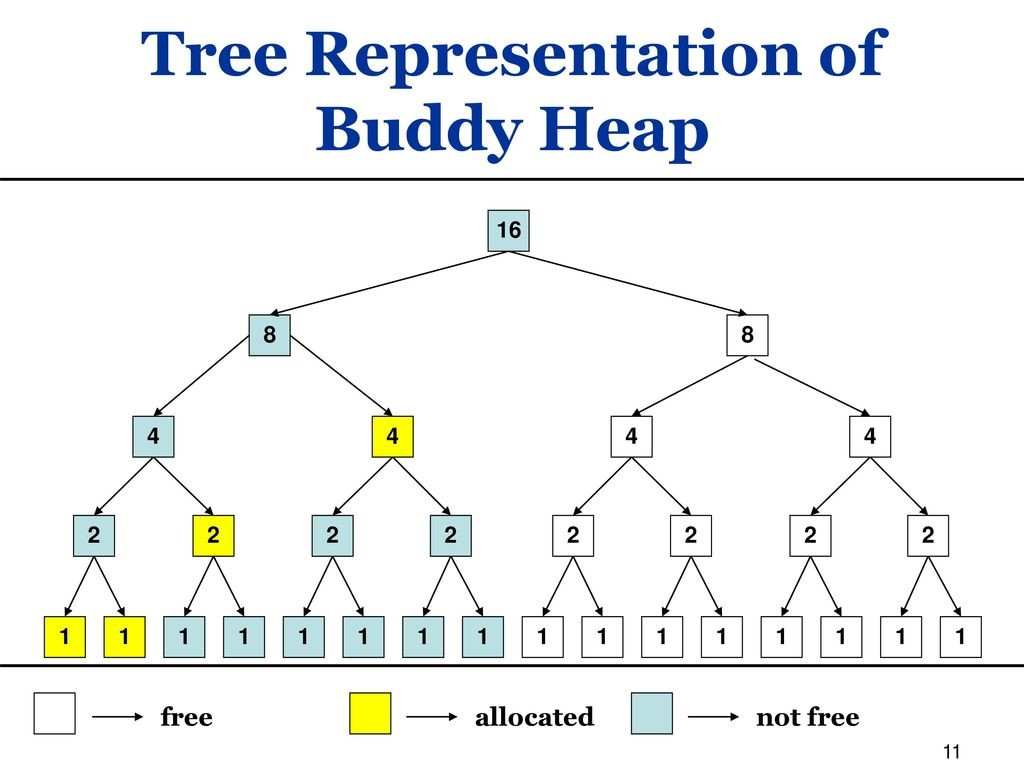
\includegraphics[scale=1.3]{imagens/BuddyHeap.jpg}
   \caption{Divisão da memória usando \emph{BuddyHeap}.\cite{arleen2018}}
   \label{fig:BuddyHeap}
\end{figure} 

O alocador \emph{kmalloc} é utilizado para solicitações de tamanho arbitrário. Assim o serviço aloca páginas inteiras sob demanda e, em seguida, divide-as em pedaços menores para satisfazer as requisições frequentes de pequenos blocos de memória. A alocação de memória utilizando esse serviço envolve determinar uma lista, entre as listas mantidas pelo \emph{kernel} das páginas alocadas, utilizando o primeiro bloco disponível na lista ou alocando uma nova página e subdividindo-a.\\ O \emph{kmalloc} não tem permissão e ou autoridade para relocar ou liberar regiões de memória já alocados mesmo que seja esta uma tratativa para uma possível falta de memória, depois de alocadas, essas regiões somente poderão ser reutilizadas mediante uma liberação explicita. Outros três subsistemas principais que tratam de sua própria gerência de páginas físicas e que interagem intimamente entre si, segundo Silberschatz(2000) são o \emph{cache} de \emph{buffers}, que é o \emph{cache} principal do \emph{kernel} para dispositivos orientados a bloco; o \emph{cache} de páginas que mantém em \emph{cache} páginas inteiras de conteúdo de arquivos, dados da rede entre outros e o sistema de memória virtual que gerencia o espaço de endereçamento virtual de cada processo \cite{Tanenbaum2016}, \cite{ufscar2019}, \cite{silberschatz2000}, \cite{stallings2004}.

\section{Memória Virtual}

O sistema de memória virtual no \emph{Linux} é responsável pela manutenção do espaço de endereçamento visível para cada processo assim sendo a criação das páginas de memória virtual sob demanda e a gerência do carregamento dessas páginas para o disco, ou o descarregamento de volta para o disco, é responsabilidade desse sistema.\\
O gerente de memória virtual mantem duas perspectivas do espaço de endereçamento de um processo sendo a primeira, é a visão lógica e a segunda a visão física de cada espaço de endereçamento \cite{ufscar2019}, \cite{silberschatz2000}, \cite{stallings2004}.\\
Na primeira instruções recebidas pelo sistema de memória virtual referentes  ao layout do espaço de endereçamento que consiste em um conjunto de regiões não superpostas, com cada uma representando um subconjunto contínuo e alinhado por página do espaço de endereçamento e sendo descrita internamente por uma única estrutura \emph{vm\_area \_struct} (é uma estrutura de dados utilizada para descrever uma área da memória virtual para um processo), que define as propriedades da região. Na segunda é armazenada uma tabela de páginas do \emph{hardware} para o processo e é gerenciada por um conjunto de rotinas.\\
 Cada \emph{vm\_area \_struct}  na descrição do espaço de endereçamento contém um campo que aponta para uma tabela de funções que implementam as funções básicas de gerência de página para qualquer região dada da memória virtual \cite{ufscar2019}, \cite{silberschatz2000}, \cite{stallings2004}.\\
No \emph{Linux} existem diversos tipos de região de memória virtual mais suas propriedades de caracterização são do tipo de armazenamento secundário associado e sua reação a escritas, as regiões de espaço de endereçamento de um processo pode ser privada ou compartilhada sendo feito um processo \emph{Copy-on-write} (é a operação onde uma região privada é copiada para uma nova região a fim de preservar essa região contra escritas a partir de outro processo) quando tentar escrever em uma região privada de outro processo, copiando o conteúdo da região para uma outra região nova e efetua as alterações na região recém-criada, preservando a região privada. Caso está escrita seja feita em região compartilhada o objeto mapeado para tal região é atualizado, de modo que as alterações ficam visíveis de imediato para todos os processos que estiverem mapeando tal objeto.\\
O \emph{Linux} cria espaços de endereçamento através de duas situações em um novo programa que é chamado solicitando ao sistema de execução um novo espaço de endereçamento, no qual o processo ao receber este espaço ele está completamente vazio, e a rotina carrega o programa para ocupar o espaço, ou quando um novo processo é criado por \emph{fork}, o que significa que uma cópia completa do espaço de endereço é criada para o processo existente \cite{ufscar2019}, \cite{silberschatz2000}, \cite{stallings2004}.


\section{Swapping e paginação}

Com uma crescente utilização da memória através de sistemas de tempo compartilhado ou computadores pessoais orientados graficamente por vezes a memória principal não possuem espaço suficiente para manter todos os processos ativos uma solução para isso é salvar parte destes processos excedentes colocando os no disco liberando assim espaço para novos processos e estes ficando em stand-by esperando serem chamados novamente. Assim sendo dependendo do \emph{hardware} duas técnicas podem ser utilizadas \cite{ufscar2019}, \cite{silberschatz2000}, \cite{stallings2004}.\\
A técnica mais simples, é o /emph{swapping} usada para algoritmos de escalonamento, baseando-se em prioridades. Se um processo de prioridade mais alta necessitar ser carregado, o gerenciador de memória poderá descarregar um outro com prioridade mais baixa para o disco, para que o de maior prioridade possa ser executado. Quando for finalizado, o processo descarregado pode então, ser carregado novamente para a memória principal. Segundo Silberschatz(2000), quando o escalonador de CPU executar um processo, ele chama o \emph{dispatcher} (também chamado de agendador de curto prazo, conforme Stallings(2004) descreve, decide qual dos processos na memória, prontos para a execução, será executado pelo processador) , que verifica se o próximo processo na fila está na memória. Se o processo não estiver na memória e não houver região de memória livre, o \emph{dispatcher} descarrega um processo que está na memória \emph{(swap out)} e carrega o processo desejado em seu lugar \emph{(swap in)}, recarregando, então, os registradores de forma usual e transferindo o controle para o processo selecionado \cite{ufscar2019}, \cite{silberschatz2000}, \cite{stallings2004}.\\
No \emph{Linux}, o processo de paginação pode ser dividido em duas seções: o algoritmo de políticas, primeiramente, que decide que páginas são gravadas no disco e quando esse processo será feito, por meio de uma versão modificada do algoritmo de relógio, que emprega um relógio de passagens múltiplas. \\
A segunda seção, é o mecanismo de paginação, que suporta tanto partições e dispositivos dedicados, quanto arquivos, sendo que no último, o processo pode ser mais lento devido ao custo adicional provocado pelo sistema de arquivos. O algoritmo utilizado para a gravação das páginas é o algoritmo \emph{next-fit}, para tentar gravar páginas em carreiras contínuas de blocos de disco, visando um melhor desempenho \cite{ufscar2019}, \cite{silberschatz2000}, \cite{stallings2004}.